% !TEX root = ../Thesis.tex

\chapter{Results}\
\label{ch:results}

Still need to run archetypes on Zurich west (ca.2h), generate radiation data for all NO-ASF cases, and run archetypes on those ca. 10h... But here are some initial graphs

\begin{figure}[h] %h can be omitted for better page layout
  \begin{center}
    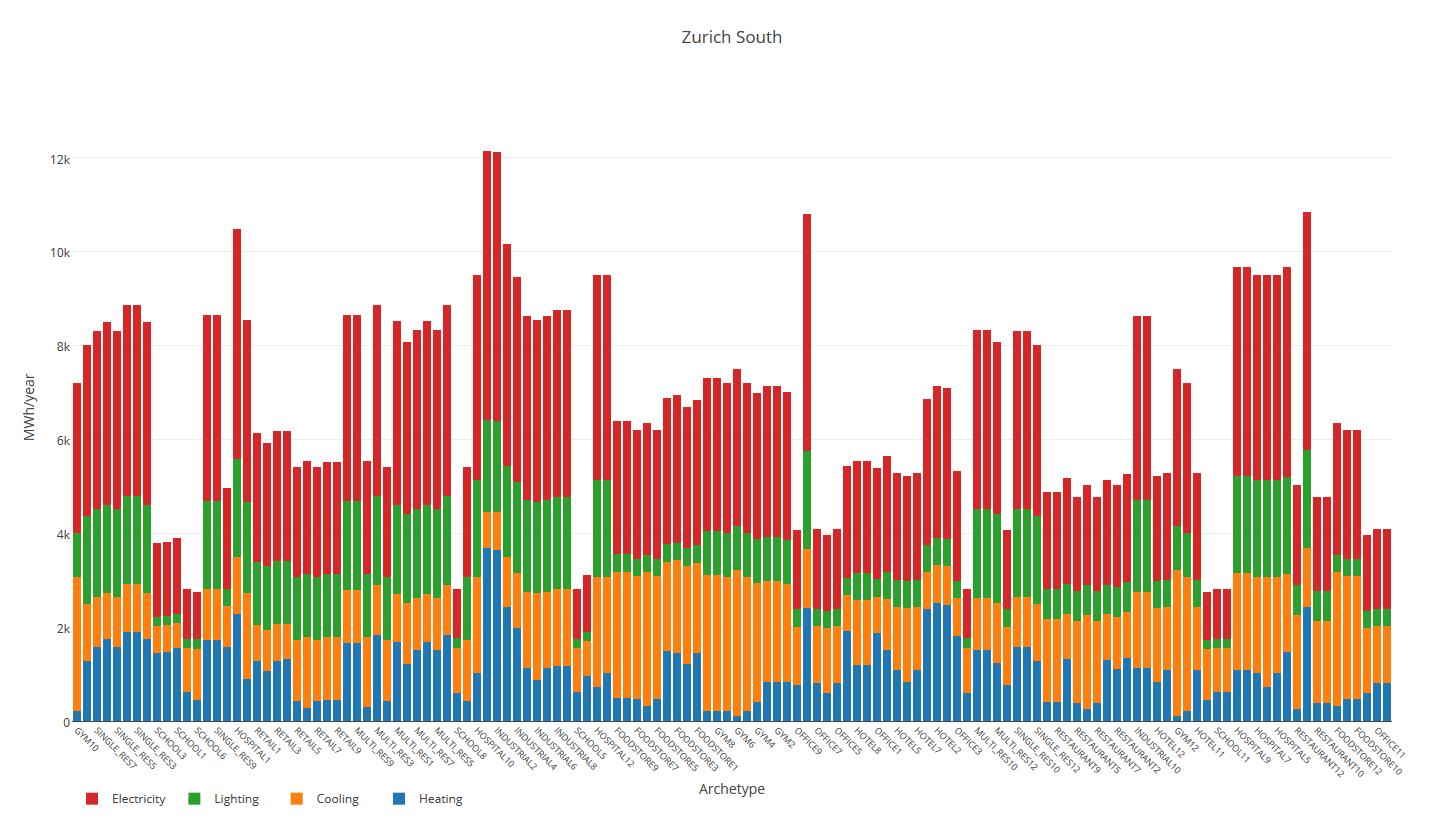
\includegraphics[width=\textwidth, trim= 0cm 0cm 0cm 0cm,clip]{zs.png}
    \caption{Archetype comparison for Zurich[South]}
    \label{fig: zs}
  \end{center} 
\end{figure}

blah\par

\begin{figure}[h] %h can be omitted for better page layout
  \begin{center}
    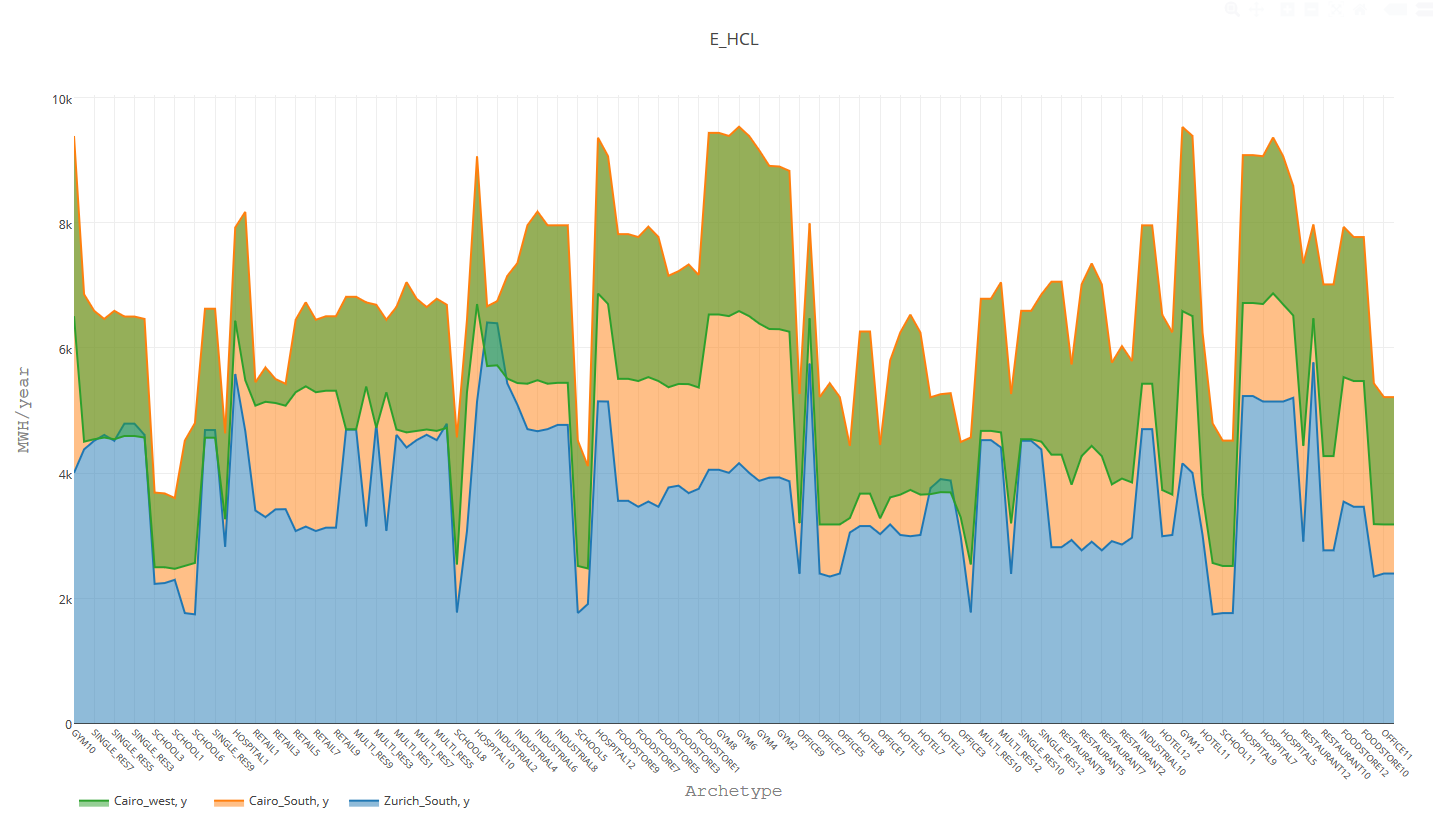
\includegraphics[width=\textwidth, trim= 0cm 0cm 0cm 0cm,clip]{hcl.png}
    \caption{Comparison of Total Energy \textit{(heating, cooling, lighting)} for the four location scenarios}
    \label{fig: ASF}
  \end{center} 
\end{figure}

blah\par

\begin{figure}[h] %h can be omitted for better page layout
  \begin{center}
    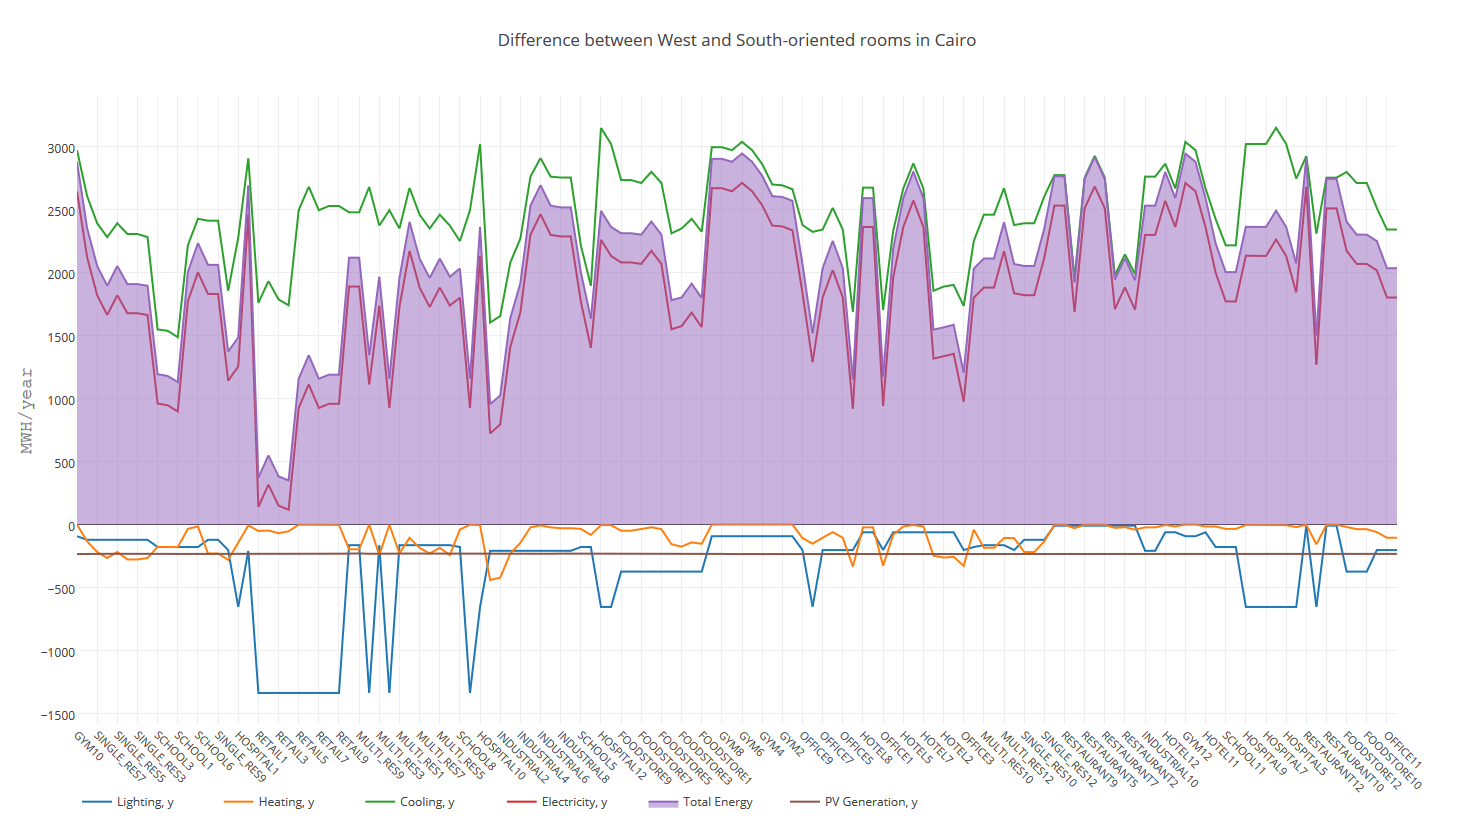
\includegraphics[width=\textwidth, trim= 0cm 0cm 0cm 0cm,clip]{west-south.png}
    \caption{\textit{Difference} between West and South oriented buildings in the Cairo case}
    \label{fig: ASF}
  \end{center} 
\end{figure}

QUOTE FROM JEREMIAS: It was possible to find the optimising configurations of the described system as well as the corresponding building energy demand. Furthermore, various influences were evaluated including sensitivities on the building orientation, the geographic location, the control strategy, and the building system parameters. For the chosen base case evaluation, energy benefits of 9\% were obtained when compared to a fixed solar facade at the most beneficial angle. The corresponding PV electricity output is able to compensate for 41\percent of the total building energy demand. The benefits are even larger for warmer regions than Zurich, as well as for buildings that have less efficient heating and cooling systems.\par